%--------------------------% 
% PREAMBLE 1 - DO NOT EDIT %
%--------------------------% 
%%%%%%%%%%%%%%%%%%%%%%%%
% PREAMBLE %%%%%%%%%%%%%
%%%%%%%%%%%%%%%%%%%%%%%%

\expandafter\gdef\csname ver@amssymb.sty\endcsname{9999/12/31}
\expandafter\gdef\csname ver@amsfonts.sty\endcsname{9999/12/31}

\documentclass[12pt,twoside]{article}

\global\expandafter\let\csname ver@amssymb.sty\endcsname\relax
\global\expandafter\let\csname ver@amsfonts.sty\endcsname\relax

\usepackage[small,bf]{caption}
\usepackage[charter]{mathdesign}
\usepackage{amsmath}
\usepackage{graphicx}
\usepackage{qtree}
\usepackage{subcaption}
\usepackage{fancyhdr}
%\usepackage{amsthm}
\usepackage{float}
\usepackage{pdflscape}
\usepackage[hidelinks]{hyperref}
\usepackage{lipsum}
\usepackage{enumitem}
\setlength{\headheight}{40pt}

\newtheorem{theorem}{Theorem}

% PAGE DIMENSIONS
\voffset=-.5in
\hoffset=-.75in
\oddsidemargin=0.65in
\evensidemargin=0.65in
\topmargin=-0.15in
\textheight=9.1in
\textwidth=6.7in

% COLOUR STUFF
\usepackage[dvipsnames]{xcolor}
\definecolor{acolor}{RGB}{118,32,43} % Colour of the article title and sections
\newcommand*{\newhref}[2]{\href{#1}{\textbf{\textcolor{acolor}{#2}}}}
\newcommand{\localtextbulletone}{\textcolor{acolor}{\raisebox{.45ex}{\rule{.6ex}{.6ex}}}}
\renewcommand{\labelitemi}{\localtextbulletone}

\usepackage{sectsty}
\sectionfont{\color{acolor}}  % sets colour of chapters
\subsectionfont{\color{acolor}}  % sets colour of sections

%\addto{\captionsenglish}{\renewcommand{\abstractname}{Summary}}
\makeatletter
\renewcommand{\maketitle}{\bgroup\setlength{\parindent}{0pt}
\begin{flushleft}
  \textbf{\@title}
  
  \@author
\end{flushleft}\egroup
}
\renewcommand{\footrulewidth}{0.4pt}% default is 0pt
\makeatother

%-----------------------------% 
% PROJECT-SPECIFIC PARAMETERS %
%-----------------------------% 
\newcommand{\thedraft}{(DRAFT)}
%\newcommand{\thedraft}{}

\newcommand{\titlestring}{Flight Route Predictive Analytics Model for Telesat LEO}
\newcommand{\theprojectnumber}{4376E-F19-TELESAT-002}
\newcommand{\theclient}{Dr. Maryam Haghighi}
\newcommand{\theshortclient}{Dr. Haghighi}
\newcommand{\theclientrole}{Manager \\ Satellite Communications Analytics}
\newcommand{\theclientaddress}{160 Elgin Street, Suite 2100 \\ Ottawa, Ontario  K2P 2P7 \\ Canada}
\newcommand{\thestudents}{Vatya Kishore, Smit Patel, Dhruv Pramod,\ }
\newcommand{\theshortstudents}{V Kishore, S Patel, D Pramod,\ }

%--------------------------% 
% PREAMBLE 2 - DO NOT EDIT %
%--------------------------%
\title{\textcolor{acolor}{\LARGE{\titlestring }}}

\author{\ \\ \normalsize{\thestudents Patrick Boily} \\ \small{Department of Mathematics and Statistics, University of Ottawa}  \\ \ \\ \today }


\renewcommand{\sectionmark}[1]{\markboth{\textsc{#1}}{}}
\newcommand{\newl}{\newline\newline}

\begin{document}


\begingroup
\let\center\flushleft
\let\endcenter\endflushleft
\maketitle
\thispagestyle{fancy}
\lhead{}
\chead{
\includegraphics[height=35pt]{Images/uOttawa}\hfill 
\includegraphics[height=35pt]{Images/dms}}
\rhead{}
\lfoot{\ }
\cfoot{\footnotesize{STEM Complex, room 541 $-$ 150 Louis-Pasteur Pvt., 
Ottawa, ON, Canada K1N 6N5 $-$ \newhref{mailto:pboily@uottawa.ca}{pboily@uottawa.ca}}}

\endgroup
\small
\tableofcontents
\newpage
\listoffigures
\newpage
\listoftables
\normalsize
\newpage\noindent

\pagestyle{fancy}
\lhead[\textsc{\titlestring\thedraft}]{\theshortstudents P Boily}
\rhead[\theshortstudents P Boily]{\leftmark}
\chead{}
\rfoot[\footnotesize\thepage]{\footnotesize{Project Number: \theprojectnumber \thedraft}}
\cfoot{}
\lfoot[\footnotesize{Project Number: \theprojectnumber  \thedraft}]{\footnotesize{\thepage}}


%-----------------%
% START OF REPORT %
%-----------------%
\section{Project Overview and Statement}
The goal of this project was to take a data set consisting of Historical Flight Path Data and  Flight Schedule, and create a predictive model that would output a time-weighted probability distribution of flight locations for each coverage area. This information can be used for future implementations of flight prediction as the current model takes into account the delays of any flight that may occur.

\subsection{Report Objectives}
This report will explore the methodology determined to create a predictive model as well as the process in creating a predictive model for flight paths and coverage areas. Whilst discussing the process of creating a training set, delay prediction, flight probability distribution, and validation, the idea of how flight routes for a given Origin-Destination pairing will be explored.
\par All the data for both the training set and analysis has been taken from the commercial/business Atlantic Flights data set provided by Dr. Haghighi.
%\begin{itemize}[noitemsep]
%\item 1
%\item 2
%\end{itemize}
%It was sad when the great ship went down \cite{ref1}. %\newl etc. 
\subsection{Background}
Telesat is a global leader in satellite operation, providing reliable and secure satellite-delivered communications solutions worldwide. They provide high value expertise and support to industry participants on a global basis. Telesat owns 16 GEO satellites, the Canadian payload on ViaSat-1 and one Phase 1 LEO satellite which is the start of Telesat’s planned advanced global LEO satellite constellation that will offer ultra-low latency, extremely high throughput, affordable broadband services.\\
Telesat is launching a state-of-the-art satellite constellation of highly advanced satellites in low-earth-orbit (LEO) that will seamlessly integrate with terrestrial networks. The global network will deliver fiber quality throughput anywhere on earth. This is a highly flexible system that dynamically allocates capacity where there’s demand, thus maximizing system efficiency. This is a future-proof solution to backhaul cellular traffic, and to provide high-speed broadband access to planes, ships and remote enterprise and government users. Capacity will be available as layer-2 connectivity for service providers to connect their end users.
\subsection{Executive Summary}
By creating this predictive analysis model, Telesat is able to take any data set with an Origin-Destination pairing, as well as a scheduled departure time, and receive back a forecasted probability distribution of flight locations in the given time interval for a day. This data can be used to gain a better idea of where satellites can be placed in advance to gain maximum coverage of an airline. 
\section{Preliminaries}\label{sec:sec3}
Figure \ref{fig:fig1} depicts a logo.

\begin{figure}[t]
\centering
    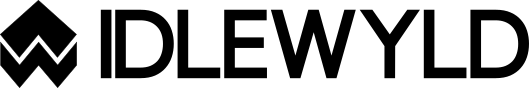
\includegraphics[width=0.67\textwidth]{Images/logo2-large.png}
  \caption[Behold, the logo.]{Behold the logo! It is quite large!}\hrule
          \label{fig:fig1}
\end{figure}

\subsection{Definitions}\label{sec:sec4}
\textbf{Origin-Destination} refers to a starting point and ending point for any given flight.
\newl \textbf{Tensor} is a mathematical object analogous to but more general than a vector, represented by an array of components that are functions of the coordinates of a space.

\subsection{Methodology}\label{sec:sec5}

\begin{figure}[htbp]
\par\medskip \centering
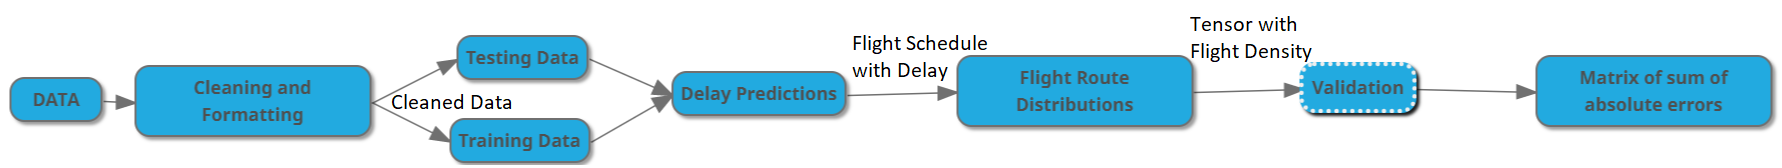
\includegraphics[width=1\textwidth]{Deliverables/Images/FlowOfCode.PNG}
\caption[Basic Flow of Program Execution]{Basic Flow of Program Execution}
\hrule
\label{fig:proex}
\end{figure}

The first step for our methodology is to clean and format the given data. The cleaned data is then split into a training set and testing set (See Section \ref{sec:sec6}). Then the delay function (See Section \ref{sec:sec7}) outputs a flight schedule with all of the predicted delays. Using this flight schedule, a three dimensional tensor is created (See Section \ref{sec:sec8}) with the location (latitude and longitude) of every flight in the schedule at five minute intervals. The tensor is then validated using the sum of absolute errors.

\section{Data Cleaning and Formatting} \label{sec:sec9}
Before any model could be built, the data needed to be cleaned and formatted for ease of use, and any anomalies needed to be removed from the data set. There were 269 flights in the data set provided whose first timestamp was recorded over 15 minutes past the actual time of departure. For the purposes of this project these flights were removed from the data set. Next all non-commercial flights were removed as majority of the flights of interest are commercial airlines and non-commercial flights may not have historical data available.\\
The data set is then reduced to only keep a few of the variables from the original data. The variables retained are: Flight ID, Origin, Destination, Filed Departure Time (Split into separate date and time columns), Actual Departure Time (Split into separate date and time columns) and the Date from the timestamps. A new index variable was created for latitude, longitude, time from the timestamp and departure time. Next, only one observation for each time index for each flight is retained. The latitude and longitude indices for every time index is the average over all unique flight id and time index. Doing so reduces the size of the dataframe by more than half. The cleaned data is then used in the next steps of the pipeline.

\section{Training Set} \label{sec:sec6}
The idea for a training set was to take 80 percent of flights between every Origin-Destination pair, and compare the predicted flight routes to the observed flight routes. Origin-Destination pairs that had 2 or less flights were not included in this training set as their flight pairings were not frequent enough to include in the set. In order to do this, a list of Origin-Destination pairs was created from which the 80 percent of flights would be extracted. Using an if-else statement inside a for loop, the flights with 2 or more origin-destination pairings could be differentiated from those with less than 2 pairings. By combining both the training data, and the testing data, a training set was formulated.  With this training set, we were able to create a foundation for our model and validations.

\section{Prediction of Delays}\label{sec:sec7}
To predict the departure delay for a flight, a function (\textbf{delay.predict}) was created that requires historical data of the flights and the schedule of the flights for which the delay is to be predicted. The schedule should specify the origin-destination pair along with the scheduled time of departure. The function first checks if the specified origin-destination pair is a part of the historical data. It then finds the distribution of delays for all the flights departing in the same hour for each origin-destination pair. It generates a random number between 0 and 1 for each flight in the schedule(\textbf{rx}), rounds it down to the closest 0.05 (\textbf{ry}) to find which quantile it belongs to. The minimum delay is set to the same quantile and the maximum delay is set to the next quantile. The predicted delay is the proportional difference between \textbf{rx} and \textbf{ry} times the length of each quantile plus the minimum delay. 
\section{Flight Probability Distribution}\label{sec:sec8}
To create a flight probability distribution, the function as mentioned in section 4 was created. With the delay prediction, as well as a training set to compare the delay prediction, a tensor was created which contained every possible flight location. A tensor is essentially a generalisation of matrices in n-dimensions, so data can be worked interchangeably. In this case the tensor was created as a "total sum". That is, it is the sum of all tensors created for each fight in the flight schedule. The tensor for each flight contains all possible routes. This allows us to see the density of planes in each 2$^\circ$ by 2$^\circ$ section of the atmosphere.\\
The results were then validated using the average sum of absolute errors for each cell summed over the 288 time intervals.
\section{Results}
Based off the training set, prediction of delays and flight probability distribution, a heat map was able to be generated, which displayed where the majority of planes would be. With this heat map, Telesat will be able to get a accurate representation of the most dense regions for flights for any given Origin-Destination pair.

\section{Next Steps and Recommendations}
This project was built with the idea that it could be used as a prototype for the real flight route prediction software. Due to the processing capabilities of the computers available to the team and the timeframe of the project, it was not possible to build a full system.\\
\textbf{Next Steps}
\begin{itemize}
    \item The delay prediction module can be improved as it currently relies on a random number generator.
    \item The flight route prediction can be improved first by increasing the size of the data set and then by using only the flights that have departed within the hour of the scheduled departure time and not all flights in the origin-destination pair.
    \item Next the expected location of the flight could be calculated using the probabilities generated in the previous step.
    \item The flight route prediction function can be further improved by using more complex algorithms rather than using the law of large numbers from probability theory.
\end{itemize}
%%%%%%%%%%%%%%%%%%%%%%%%
% REFERENCES %%%%%%%%%%%
%%%%%%%%%%%%%%%%%%%%%%%%
\begin{thebibliography}{99}
\bibitem{ref1} Arvix [2019], A Machine Learning Approach to Air Traffic Route Choice Modelling, {\it https://arxiv.org/ftp/arxiv/papers/1802/1802.06588.pdf}
\bibitem{ref2} Arvix [2019], Predicting Aircraft Trajectories: A Deep Generative Convolutional Recurrent Neural Networks Approach, {\it https://arxiv.org/ftp/arxiv/papers/1812/1812.11670.pdf}
\bibitem{ref3} Bayes, T. [1763], An Essay towards solving a Problem in the Doctrine of Chances, {\it Phil. Trans. Royal Society London}.
\bibitem{ref4} CiteSeeRX [2019], Estimating Flight Departure Delay Distributions —A Statistical Approach With Long-term Trend and Short-term Pattern, {\it http://citeseerx.ist.psu.edu/viewdoc/download?doi=10.1.1.132.1147\&rep=rep1\&type=pdf}
\bibitem{ref5} FlightRadar24 [2019], Live Air Traffic, {\it https://www.flightradar24.com/data/flights}
\bibitem{ref6} FlightAware [2019], Live Flight Tracking, {\it https://flightaware.com}
\bibitem{ref7} The Denver Post [2019], Get ready for the 19-hour flight: Qantas sets record for world’s longest nonstop flight, {\it https://www.denverpost.com/2019/10/20/world-longest-nonstop-flight-qantas/}
\end{thebibliography}




\end{document}
